\documentclass[tikz,border=2pt]{standalone}
\usepackage{amsmath}
\usepackage[T1]{fontenc}
\usepackage[tt=false, type1=true]{libertine}
\usepackage[varqu]{zi4}
\usepackage[libertine]{newtxmath}
\usetikzlibrary{positioning,arrows.meta,fit,backgrounds,calc}

\newcommand{\Z}{\mathbb{Z}}

\definecolor{ink}{HTML}{16191D}
\definecolor{accent}{HTML}{1F4E79}
\definecolor{accentsoft}{HTML}{E8EEF4}
\definecolor{accentwarm}{HTML}{9A5B00}
\definecolor{accentplum}{HTML}{8E2F5F}
\definecolor{muted}{HTML}{5B6470}
\definecolor{hairline}{HTML}{C9CFD6}

\tikzset{
    house/.style={
    >={Stealth[length=2.1mm, width=1.6mm]},
    line width=0.5pt,
    node distance=9mm and 15mm,
    every node/.style={font=\small},
  },
    box/.style={
    draw=ink, line width=0.5pt, rounded corners=1.5pt,
    inner xsep=6pt, inner ysep=4pt, align=center,
  },
    boxhi/.style={box, draw=accent, fill=accentsoft, text=ink},
    boxdim/.style={box, draw=hairline, text=muted},
    flow/.style={->, draw=ink},
  flowdim/.style={->, draw=hairline},
  lbl/.style={font=\footnotesize\itshape, text=accent, inner sep=2pt},
  lbldim/.style={font=\footnotesize, text=muted, inner sep=2pt},
    group/.style={draw=hairline, dashed, rounded corners=2pt, inner sep=7pt},
}

\newcommand{\ket}[1]{\lvert #1\rangle}
\newcommand{\bra}[1]{\langle #1\rvert}

\begin{document}
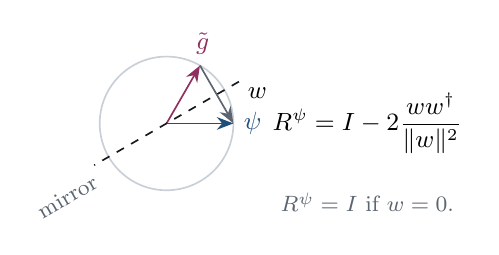
\begin{tikzpicture}[house, semithick, font=\small]
    \begin{scope}[shift={(1.5,3.3)}, scale=0.653]
    \def\rr{1.3}
    \draw[hairline] (0,0) circle (\rr);
    \draw[->, accent] (0,0) -- (\rr,0);
    \node[text=accent, anchor=west, inner sep=2pt] at (\rr+0.08,0) {$\psi$};
    \draw[->, accentplum] (0,0) -- (60:\rr);
    \node[text=accentplum, anchor=south, inner sep=2pt] at (60:\rr+0.1) {$\tilde g$};
    \draw[ink, dashed] (30:1.25*\rr) -- (210:1.25*\rr);
    \draw[->, muted] (60:\rr) -- (\rr,0);
    \node[anchor=west, inner sep=2pt] at (1.12*\rr,0.45*\rr) {$w$};
    \node[font=\footnotesize, text=muted, rotate=30, anchor=north east, inner sep=2pt] at (210:1.25*\rr) {mirror};
  \end{scope}
    \node at (4.05,3.3) {$R^{\psi}=I-2\dfrac{ww^\dagger}{\|w\|^2}$};
  \node[font=\footnotesize, text=muted] at (4.05,2.3) {$R^{\psi}=I$ if $w=0$.};
\end{tikzpicture}
\end{document}
